\documentclass[twoside]{book}

% Packages required by doxygen
\usepackage{fixltx2e}
\usepackage{calc}
\usepackage{doxygen}
\usepackage[export]{adjustbox} % also loads graphicx
\usepackage{graphicx}
\usepackage[utf8]{inputenc}
\usepackage{makeidx}
\usepackage{multicol}
\usepackage{multirow}
\PassOptionsToPackage{warn}{textcomp}
\usepackage{textcomp}
\usepackage[nointegrals]{wasysym}
\usepackage[table]{xcolor}

% Font selection
\usepackage[T1]{fontenc}
\usepackage[scaled=.90]{helvet}
\usepackage{courier}
\usepackage{amssymb}
\usepackage{sectsty}
\renewcommand{\familydefault}{\sfdefault}
\allsectionsfont{%
  \fontseries{bc}\selectfont%
  \color{darkgray}%
}
\renewcommand{\DoxyLabelFont}{%
  \fontseries{bc}\selectfont%
  \color{darkgray}%
}
\newcommand{\+}{\discretionary{\mbox{\scriptsize$\hookleftarrow$}}{}{}}

% Page & text layout
\usepackage{geometry}
\geometry{%
  a4paper,%
  top=2.5cm,%
  bottom=2.5cm,%
  left=2.5cm,%
  right=2.5cm%
}
\tolerance=750
\hfuzz=15pt
\hbadness=750
\setlength{\emergencystretch}{15pt}
\setlength{\parindent}{0cm}
\setlength{\parskip}{3ex plus 2ex minus 2ex}
\makeatletter
\renewcommand{\paragraph}{%
  \@startsection{paragraph}{4}{0ex}{-1.0ex}{1.0ex}{%
    \normalfont\normalsize\bfseries\SS@parafont%
  }%
}
\renewcommand{\subparagraph}{%
  \@startsection{subparagraph}{5}{0ex}{-1.0ex}{1.0ex}{%
    \normalfont\normalsize\bfseries\SS@subparafont%
  }%
}
\makeatother

% Headers & footers
\usepackage{fancyhdr}
\pagestyle{fancyplain}
\fancyhead[LE]{\fancyplain{}{\bfseries\thepage}}
\fancyhead[CE]{\fancyplain{}{}}
\fancyhead[RE]{\fancyplain{}{\bfseries\leftmark}}
\fancyhead[LO]{\fancyplain{}{\bfseries\rightmark}}
\fancyhead[CO]{\fancyplain{}{}}
\fancyhead[RO]{\fancyplain{}{\bfseries\thepage}}
\fancyfoot[LE]{\fancyplain{}{}}
\fancyfoot[CE]{\fancyplain{}{}}
\fancyfoot[RE]{\fancyplain{}{\bfseries\scriptsize Generated by Doxygen }}
\fancyfoot[LO]{\fancyplain{}{\bfseries\scriptsize Generated by Doxygen }}
\fancyfoot[CO]{\fancyplain{}{}}
\fancyfoot[RO]{\fancyplain{}{}}
\renewcommand{\footrulewidth}{0.4pt}
\renewcommand{\chaptermark}[1]{%
  \markboth{#1}{}%
}
\renewcommand{\sectionmark}[1]{%
  \markright{\thesection\ #1}%
}

% Indices & bibliography
\usepackage{natbib}
\usepackage[titles]{tocloft}
\setcounter{tocdepth}{3}
\setcounter{secnumdepth}{5}
\makeindex

% Hyperlinks (required, but should be loaded last)
\usepackage{ifpdf}
\ifpdf
  \usepackage[pdftex,pagebackref=true]{hyperref}
\else
  \usepackage[ps2pdf,pagebackref=true]{hyperref}
\fi
\hypersetup{%
  colorlinks=true,%
  linkcolor=blue,%
  citecolor=blue,%
  unicode%
}

% Custom commands
\newcommand{\clearemptydoublepage}{%
  \newpage{\pagestyle{empty}\cleardoublepage}%
}

\usepackage{caption}
\captionsetup{labelsep=space,justification=centering,font={bf},singlelinecheck=off,skip=4pt,position=top}

%===== C O N T E N T S =====

\begin{document}

% Titlepage & ToC
\hypersetup{pageanchor=false,
             bookmarksnumbered=true,
             pdfencoding=unicode
            }
\pagenumbering{roman}
\begin{titlepage}
\vspace*{7cm}
\begin{center}%
{\Large Machine Gaming \\[1ex]\large 1.\+0 }\\
\vspace*{1cm}
{\large Generated by Doxygen 1.8.11}\\
\end{center}
\end{titlepage}
\clearemptydoublepage
\tableofcontents
\clearemptydoublepage
\pagenumbering{arabic}
\hypersetup{pageanchor=true}

%--- Begin generated contents ---
\chapter{Machine\+Gaming}
\label{index}\hypertarget{index}{}\subsubsection*{Description}

Neural Network learning how to play Asteroids. Project for advanced programming classes.

\subsubsection*{Linux installation}


\begin{DoxyEnumerate}
\item Download and unpack or clone repository to desired location.
\item Open Machine\+Gaming folder.
\item To install type\+: sh install.\+sh
\item To run tests go to bin directory and type\+: make test
\item To run asteroids demo type\+: sh run.\+sh 
\end{DoxyEnumerate}
\chapter{Hierarchical Index}
\section{Class Hierarchy}
This inheritance list is sorted roughly, but not completely, alphabetically\+:\begin{DoxyCompactList}
\item \contentsline{section}{Coordinates.\+Coordinates}{\pageref{classCoordinates_1_1Coordinates}}{}
\item \contentsline{section}{Counter$<$ T $>$}{\pageref{classCounter}}{}
\item \contentsline{section}{Counter$<$ Connection $>$}{\pageref{classCounter}}{}
\begin{DoxyCompactList}
\item \contentsline{section}{Connection}{\pageref{classConnection}}{}
\end{DoxyCompactList}
\item \contentsline{section}{Counter$<$ Neuron $>$}{\pageref{classCounter}}{}
\begin{DoxyCompactList}
\item \contentsline{section}{Neuron}{\pageref{classNeuron}}{}
\end{DoxyCompactList}
\item \contentsline{section}{Evolutionary\+Algorithm}{\pageref{classEvolutionaryAlgorithm}}{}
\item \contentsline{section}{Evolutionary\+Algorithm\+Parameters}{\pageref{structEvolutionaryAlgorithmParameters}}{}
\item \contentsline{section}{Evolutionary\+Algorithm\+Wrapper}{\pageref{classEvolutionaryAlgorithmWrapper}}{}
\item \contentsline{section}{Game\+Controller.\+Game\+Controller}{\pageref{classGameController_1_1GameController}}{}
\item \contentsline{section}{Game\+Window.\+Game\+Window}{\pageref{classGameWindow_1_1GameWindow}}{}
\item \contentsline{section}{Gene}{\pageref{classGene}}{}
\begin{DoxyCompactList}
\item \contentsline{section}{Connection}{\pageref{classConnection}}{}
\item \contentsline{section}{Neuron}{\pageref{classNeuron}}{}
\end{DoxyCompactList}
\item \contentsline{section}{Genome}{\pageref{classGenome}}{}
\item \contentsline{section}{Genotype$<$ T $>$}{\pageref{classGenotype}}{}
\item \contentsline{section}{Genotype$<$ Connection $>$}{\pageref{classGenotype}}{}
\item \contentsline{section}{Genotype$<$ Neuron $>$}{\pageref{classGenotype}}{}
\item \contentsline{section}{Machine\+Gaming\+Controller.\+Machine\+Gaming\+Controller}{\pageref{classMachineGamingController_1_1MachineGamingController}}{}
\item \contentsline{section}{Neural\+Network}{\pageref{classNeuralNetwork}}{}
\item \contentsline{section}{Neural\+Network\+Wrapper}{\pageref{classNeuralNetworkWrapper}}{}
\item \contentsline{section}{Phenome}{\pageref{classPhenome}}{}
\item \contentsline{section}{Random}{\pageref{classRandom}}{}
\item Sprite\begin{DoxyCompactList}
\item \contentsline{section}{Moving\+Object.\+Moving\+Object}{\pageref{classMovingObject_1_1MovingObject}}{}
\begin{DoxyCompactList}
\item \contentsline{section}{Asteroid.\+Asteroid}{\pageref{classAsteroid_1_1Asteroid}}{}
\item \contentsline{section}{Asteroid.\+Asteroid}{\pageref{classAsteroid_1_1Asteroid}}{}
\item \contentsline{section}{Missile.\+Missile}{\pageref{classMissile_1_1Missile}}{}
\item \contentsline{section}{Missile.\+Missile}{\pageref{classMissile_1_1Missile}}{}
\item \contentsline{section}{Spaceship.\+Spaceship}{\pageref{classSpaceship_1_1Spaceship}}{}
\item \contentsline{section}{Spaceship.\+Spaceship}{\pageref{classSpaceship_1_1Spaceship}}{}
\end{DoxyCompactList}
\item \contentsline{section}{Moving\+Object.\+Moving\+Object}{\pageref{classMovingObject_1_1MovingObject}}{}
\end{DoxyCompactList}
\item Tk\begin{DoxyCompactList}
\item \contentsline{section}{Machine\+Gaming\+Window.\+Machine\+Gaming}{\pageref{classMachineGamingWindow_1_1MachineGaming}}{}
\item \contentsline{section}{Machine\+Gaming\+Window.\+Machine\+Gaming\+Window}{\pageref{classMachineGamingWindow_1_1MachineGamingWindow}}{}
\end{DoxyCompactList}
\item \contentsline{section}{Vector.\+Vector}{\pageref{classVector_1_1Vector}}{}
\end{DoxyCompactList}

\chapter{Class Index}
\section{Class List}
Here are the classes, structs, unions and interfaces with brief descriptions\+:\begin{DoxyCompactList}
\item\contentsline{section}{\hyperlink{classAsteroid_1_1Asteroid}{Asteroid.\+Asteroid} }{\pageref{classAsteroid_1_1Asteroid}}{}
\item\contentsline{section}{\hyperlink{classConnection}{Connection} \\*Represents connection between neurons }{\pageref{classConnection}}{}
\item\contentsline{section}{\hyperlink{classCoordinates_1_1Coordinates}{Coordinates.\+Coordinates} }{\pageref{classCoordinates_1_1Coordinates}}{}
\item\contentsline{section}{\hyperlink{classCounter}{Counter$<$ T $>$} \\*Template class used to count genes }{\pageref{classCounter}}{}
\item\contentsline{section}{\hyperlink{classEvolutionaryAlgorithm}{Evolutionary\+Algorithm} \\*Main library class controlling evolutionary algorithm process }{\pageref{classEvolutionaryAlgorithm}}{}
\item\contentsline{section}{\hyperlink{structEvolutionaryAlgorithmParameters}{Evolutionary\+Algorithm\+Parameters} \\*Parameters defining evolutionary algorithm }{\pageref{structEvolutionaryAlgorithmParameters}}{}
\item\contentsline{section}{\hyperlink{classEvolutionaryAlgorithmWrapper}{Evolutionary\+Algorithm\+Wrapper} \\*Wrapper for \hyperlink{classEvolutionaryAlgorithm}{Evolutionary\+Algorithm} }{\pageref{classEvolutionaryAlgorithmWrapper}}{}
\item\contentsline{section}{\hyperlink{classGameController_1_1GameController}{Game\+Controller.\+Game\+Controller} }{\pageref{classGameController_1_1GameController}}{}
\item\contentsline{section}{\hyperlink{classGameWindow_1_1GameWindow}{Game\+Window.\+Game\+Window} }{\pageref{classGameWindow_1_1GameWindow}}{}
\item\contentsline{section}{\hyperlink{classGene}{Gene} \\*Class representing gene }{\pageref{classGene}}{}
\item\contentsline{section}{\hyperlink{classGenome}{Genome} \\*Represents genome }{\pageref{classGenome}}{}
\item\contentsline{section}{\hyperlink{classGenotype}{Genotype$<$ T $>$} \\*Represents genotype }{\pageref{classGenotype}}{}
\item\contentsline{section}{\hyperlink{classMachineGamingController_1_1MachineGamingController}{Machine\+Gaming\+Controller.\+Machine\+Gaming\+Controller} }{\pageref{classMachineGamingController_1_1MachineGamingController}}{}
\item\contentsline{section}{\hyperlink{classMachineGamingWindow_1_1MachineGamingWindow}{Machine\+Gaming\+Window.\+Machine\+Gaming\+Window} }{\pageref{classMachineGamingWindow_1_1MachineGamingWindow}}{}
\item\contentsline{section}{\hyperlink{classMissile_1_1Missile}{Missile.\+Missile} }{\pageref{classMissile_1_1Missile}}{}
\item\contentsline{section}{\hyperlink{classMovingObject_1_1MovingObject}{Moving\+Object.\+Moving\+Object} }{\pageref{classMovingObject_1_1MovingObject}}{}
\item\contentsline{section}{\hyperlink{classNeuralNetwork}{Neural\+Network} \\*Represents neural network -\/ multilayer perceptron }{\pageref{classNeuralNetwork}}{}
\item\contentsline{section}{\hyperlink{classNeuralNetworkWrapper}{Neural\+Network\+Wrapper} \\*Wrapper for \hyperlink{classNeuralNetwork}{Neural\+Network} }{\pageref{classNeuralNetworkWrapper}}{}
\item\contentsline{section}{\hyperlink{classNeuron}{Neuron} \\*Represents network neurons }{\pageref{classNeuron}}{}
\item\contentsline{section}{\hyperlink{classPhenome}{Phenome} \\*Represents phenome }{\pageref{classPhenome}}{}
\item\contentsline{section}{\hyperlink{classRandom}{Random} \\*Basic random number generator }{\pageref{classRandom}}{}
\item\contentsline{section}{\hyperlink{classSpaceship_1_1Spaceship}{Spaceship.\+Spaceship} }{\pageref{classSpaceship_1_1Spaceship}}{}
\item\contentsline{section}{\hyperlink{classVector_1_1Vector}{Vector.\+Vector} }{\pageref{classVector_1_1Vector}}{}
\end{DoxyCompactList}

\chapter{Class Documentation}
\hypertarget{classAsteroid_1_1Asteroid}{}\section{Asteroid.\+Asteroid Class Reference}
\label{classAsteroid_1_1Asteroid}\index{Asteroid.\+Asteroid@{Asteroid.\+Asteroid}}


Inheritance diagram for Asteroid.\+Asteroid\+:
\nopagebreak
\begin{figure}[H]
\begin{center}
\leavevmode
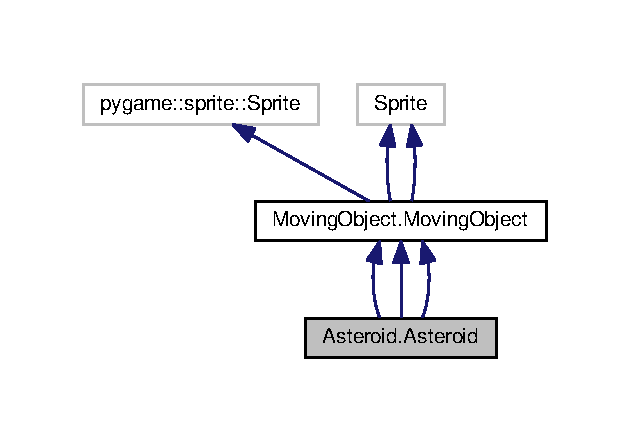
\includegraphics[width=220pt]{classAsteroid_1_1Asteroid__inherit__graph}
\end{center}
\end{figure}


Collaboration diagram for Asteroid.\+Asteroid\+:
\nopagebreak
\begin{figure}[H]
\begin{center}
\leavevmode
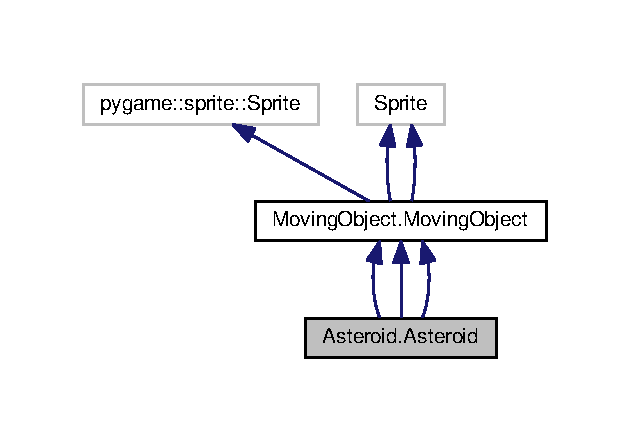
\includegraphics[width=220pt]{classAsteroid_1_1Asteroid__coll__graph}
\end{center}
\end{figure}
\subsection*{Public Member Functions}
\begin{DoxyCompactItemize}
\item 
def {\bfseries \+\_\+\+\_\+init\+\_\+\+\_\+} (self, coordinates, velocity=\hyperlink{classVector_1_1Vector}{Vector}(0, 0), scale=0.\+10, rotation\+\_\+rate=-\/0.\+5)\hypertarget{classAsteroid_1_1Asteroid_a97fe00ef73eaa80de7eec57530565e7c}{}\label{classAsteroid_1_1Asteroid_a97fe00ef73eaa80de7eec57530565e7c}

\item 
def {\bfseries update} (self, surface)\hypertarget{classAsteroid_1_1Asteroid_ac5a9f9ae0dfd3ff4aa2dabfdd820ebd1}{}\label{classAsteroid_1_1Asteroid_ac5a9f9ae0dfd3ff4aa2dabfdd820ebd1}

\item 
def {\bfseries move} (self)\hypertarget{classAsteroid_1_1Asteroid_af44489831e21c1caa55035370f671d41}{}\label{classAsteroid_1_1Asteroid_af44489831e21c1caa55035370f671d41}

\end{DoxyCompactItemize}
\subsection*{Public Attributes}
\begin{DoxyCompactItemize}
\item 
{\bfseries direction}\hypertarget{classAsteroid_1_1Asteroid_a0a8ab6e30ef6f80384878b4eb4e60d25}{}\label{classAsteroid_1_1Asteroid_a0a8ab6e30ef6f80384878b4eb4e60d25}

\end{DoxyCompactItemize}


The documentation for this class was generated from the following file\+:\begin{DoxyCompactItemize}
\item 
src/\+Asteroids/Asteroid.\+py\end{DoxyCompactItemize}

\hypertarget{classConnection}{}\section{Connection Class Reference}
\label{classConnection}\index{Connection@{Connection}}


Represents connection between neurons.  




{\ttfamily \#include $<$Connection.\+h$>$}



Inheritance diagram for Connection\+:\nopagebreak
\begin{figure}[H]
\begin{center}
\leavevmode
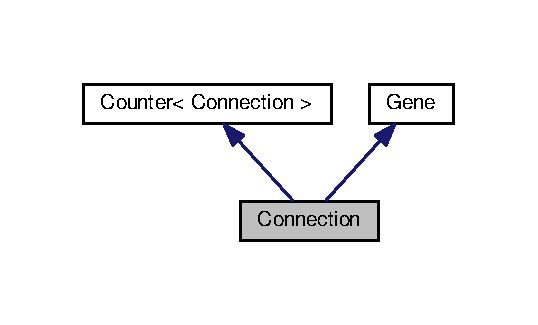
\includegraphics[width=258pt]{classConnection__inherit__graph}
\end{center}
\end{figure}


Collaboration diagram for Connection\+:\nopagebreak
\begin{figure}[H]
\begin{center}
\leavevmode
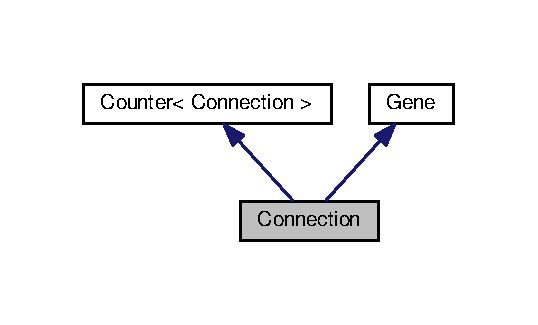
\includegraphics[width=258pt]{classConnection__coll__graph}
\end{center}
\end{figure}


\subsection{Detailed Description}
Represents connection between neurons. 

It provides \hyperlink{classGene}{Gene} methods. It is stored in \hyperlink{classGenotype}{Genotype} and when needed \hyperlink{classPhenome}{Phenome} connection matrices are built using it. \begin{DoxyAuthor}{Author}
Jakub Fajkowski 
\end{DoxyAuthor}


The documentation for this class was generated from the following files\+:\begin{DoxyCompactItemize}
\item 
src/\+A\+I/Connection.\+h\item 
src/\+A\+I/Connection.\+cc\end{DoxyCompactItemize}

\hypertarget{classCoordinates_1_1Coordinates}{}\section{Coordinates.\+Coordinates Class Reference}
\label{classCoordinates_1_1Coordinates}\index{Coordinates.\+Coordinates@{Coordinates.\+Coordinates}}


Class representing coordinates of the object.  




\subsection{Detailed Description}
Class representing coordinates of the object. 

\begin{DoxyAuthor}{Author}
Piotr Truszczynski 
\end{DoxyAuthor}


The documentation for this class was generated from the following file\+:\begin{DoxyCompactItemize}
\item 
src/\+Asteroids/Coordinates.\+py\end{DoxyCompactItemize}

\hypertarget{classCounter}{}\section{Counter$<$ T $>$ Class Template Reference}
\label{classCounter}\index{Counter$<$ T $>$@{Counter$<$ T $>$}}


Template class used to count genes.  




{\ttfamily \#include $<$Counter.\+hpp$>$}



\subsection{Detailed Description}
\subsubsection*{template$<$typename T$>$\\*
class Counter$<$ T $>$}

Template class used to count genes. 

It helps to assign id numbers to genes providing independent counters for Connections and Neurons. \begin{DoxyAuthor}{Author}
Jakub Fajkowski 
\end{DoxyAuthor}


The documentation for this class was generated from the following file\+:\begin{DoxyCompactItemize}
\item 
src/\+A\+I/Counter.\+hpp\end{DoxyCompactItemize}

\hypertarget{classEvolutionaryAlgorithm}{}\section{Evolutionary\+Algorithm Class Reference}
\label{classEvolutionaryAlgorithm}\index{Evolutionary\+Algorithm@{Evolutionary\+Algorithm}}


Main library class controlling evolutionary algorithm process.  




{\ttfamily \#include $<$Evolutionary\+Algorithm.\+h$>$}

\subsection*{Public Member Functions}
\begin{DoxyCompactItemize}
\item 
{\bfseries Evolutionary\+Algorithm} (\hyperlink{structEvolutionaryAlgorithmParameters}{Evolutionary\+Algorithm\+Parameters} p)\hypertarget{classEvolutionaryAlgorithm_a5f4f99ef49165b6db8247ca1fcd1cd3d}{}\label{classEvolutionaryAlgorithm_a5f4f99ef49165b6db8247ca1fcd1cd3d}

\item 
{\bfseries Evolutionary\+Algorithm} (const \hyperlink{classEvolutionaryAlgorithm}{Evolutionary\+Algorithm} \&eA)\hypertarget{classEvolutionaryAlgorithm_a77d812bbcecd525115d2345f1828f312}{}\label{classEvolutionaryAlgorithm_a77d812bbcecd525115d2345f1828f312}

\item 
void {\bfseries save} (std\+::string path)\hypertarget{classEvolutionaryAlgorithm_a9c13bb160c25c7b2023734d22daf33ee}{}\label{classEvolutionaryAlgorithm_a9c13bb160c25c7b2023734d22daf33ee}

\item 
void {\bfseries load} (std\+::string path)\hypertarget{classEvolutionaryAlgorithm_a847aef6411699b63a823001e92305db6}{}\label{classEvolutionaryAlgorithm_a847aef6411699b63a823001e92305db6}

\item 
P\+Neural\+Network \hyperlink{classEvolutionaryAlgorithm_ad6d0bdc4039cabff7a43e90d7ed97fa6}{get\+Next} ()
\item 
int {\bfseries get\+Current\+Network} () const \hypertarget{classEvolutionaryAlgorithm_a2eef3971fd1a53f3b468ee7c309b5a46}{}\label{classEvolutionaryAlgorithm_a2eef3971fd1a53f3b468ee7c309b5a46}

\item 
int {\bfseries get\+Current\+Generation} () const \hypertarget{classEvolutionaryAlgorithm_a3f0067ea6652ad71070631bf713b40fe}{}\label{classEvolutionaryAlgorithm_a3f0067ea6652ad71070631bf713b40fe}

\item 
const Neural\+Networks \& {\bfseries get\+Population} () const \hypertarget{classEvolutionaryAlgorithm_a97ed735aa801a51f23907eafb7c53637}{}\label{classEvolutionaryAlgorithm_a97ed735aa801a51f23907eafb7c53637}

\item 
int {\bfseries get\+Population\+Size} () const \hypertarget{classEvolutionaryAlgorithm_ac024638cfcde77429db547b329dfe56b}{}\label{classEvolutionaryAlgorithm_ac024638cfcde77429db547b329dfe56b}

\item 
int {\bfseries get\+Children\+Bred\+Per\+Generation} () const \hypertarget{classEvolutionaryAlgorithm_a014905a4ac30a361cda30a63479e5dd3}{}\label{classEvolutionaryAlgorithm_a014905a4ac30a361cda30a63479e5dd3}

\item 
double {\bfseries get\+Crossover\+Probability} () const \hypertarget{classEvolutionaryAlgorithm_ad284d6b6bcb6b1278f0d67ed53241901}{}\label{classEvolutionaryAlgorithm_ad284d6b6bcb6b1278f0d67ed53241901}

\item 
double {\bfseries get\+Mutation\+Probability} () const \hypertarget{classEvolutionaryAlgorithm_a80d717262bfe9fa36151750619cd2e85}{}\label{classEvolutionaryAlgorithm_a80d717262bfe9fa36151750619cd2e85}

\item 
int {\bfseries get\+Hidden\+Layers} () const \hypertarget{classEvolutionaryAlgorithm_a2bc50ae3e41c3874fc8d1dfb054e365b}{}\label{classEvolutionaryAlgorithm_a2bc50ae3e41c3874fc8d1dfb054e365b}

\item 
double {\bfseries get\+Weight\+Variance} () const \hypertarget{classEvolutionaryAlgorithm_aa575d0aa5378fb0cbde7d35fc2b61b93}{}\label{classEvolutionaryAlgorithm_aa575d0aa5378fb0cbde7d35fc2b61b93}

\end{DoxyCompactItemize}
\subsection*{Friends}
\begin{DoxyCompactItemize}
\item 
class {\bfseries boost\+::serialization\+::access}\hypertarget{classEvolutionaryAlgorithm_ac98d07dd8f7b70e16ccb9a01abf56b9c}{}\label{classEvolutionaryAlgorithm_ac98d07dd8f7b70e16ccb9a01abf56b9c}

\end{DoxyCompactItemize}


\subsection{Detailed Description}
Main library class controlling evolutionary algorithm process. 

Stores collection of neural networks and using \hyperlink{structEvolutionaryAlgorithmParameters}{Evolutionary\+Algorithm\+Parameters} decides whether it should crossover or mutate individuals. User can determine shape of neural networks, crossover and mutation probabilities, weight variance, population size and how many children should be bred per generation. \begin{DoxyAuthor}{Authors}
Piotr Truszczynski, Jakub Fajkowski 
\end{DoxyAuthor}


\subsection{Member Function Documentation}
\index{Evolutionary\+Algorithm@{Evolutionary\+Algorithm}!get\+Next@{get\+Next}}
\index{get\+Next@{get\+Next}!Evolutionary\+Algorithm@{Evolutionary\+Algorithm}}
\subsubsection[{\texorpdfstring{get\+Next()}{getNext()}}]{\setlength{\rightskip}{0pt plus 5cm}P\+Neural\+Network Evolutionary\+Algorithm\+::get\+Next (
\begin{DoxyParamCaption}
{}
\end{DoxyParamCaption}
)}\hypertarget{classEvolutionaryAlgorithm_ad6d0bdc4039cabff7a43e90d7ed97fa6}{}\label{classEvolutionaryAlgorithm_ad6d0bdc4039cabff7a43e90d7ed97fa6}
The result of this method depends on current\+\_\+network\+\_\+ counter. If current network number is equal to population size -\/ there are some offsprings added to population vector. After that algorithm will return children networks. If the last child is selected, counter resets and the weakest networks are killed. \begin{DoxyReturn}{Returns}
Current neural network chosen by algorithm. 
\end{DoxyReturn}


The documentation for this class was generated from the following files\+:\begin{DoxyCompactItemize}
\item 
src/\+A\+I/Evolutionary\+Algorithm.\+h\item 
src/\+A\+I/Evolutionary\+Algorithm.\+cc\end{DoxyCompactItemize}

\hypertarget{structEvolutionaryAlgorithmParameters}{}\section{Evolutionary\+Algorithm\+Parameters Struct Reference}
\label{structEvolutionaryAlgorithmParameters}\index{Evolutionary\+Algorithm\+Parameters@{Evolutionary\+Algorithm\+Parameters}}


Parameters defining evolutionary algorithm.  




{\ttfamily \#include $<$Evolutionary\+Algorithm.\+h$>$}



\subsection{Detailed Description}
Parameters defining evolutionary algorithm. 

\begin{DoxyAuthor}{Authors}
Piotr Truszczynski, Jakub Fajkowski 
\end{DoxyAuthor}


The documentation for this struct was generated from the following file\+:\begin{DoxyCompactItemize}
\item 
src/\+A\+I/Evolutionary\+Algorithm.\+h\end{DoxyCompactItemize}

\hypertarget{classEvolutionaryAlgorithmWrapper}{}\section{Evolutionary\+Algorithm\+Wrapper Class Reference}
\label{classEvolutionaryAlgorithmWrapper}\index{Evolutionary\+Algorithm\+Wrapper@{Evolutionary\+Algorithm\+Wrapper}}


Wrapper for \hyperlink{classEvolutionaryAlgorithm}{Evolutionary\+Algorithm}.  




{\ttfamily \#include $<$Evolutionary\+Algorithm\+Wrapper.\+h$>$}



\subsection{Detailed Description}
Wrapper for \hyperlink{classEvolutionaryAlgorithm}{Evolutionary\+Algorithm}. 

It makes \hyperlink{classEvolutionaryAlgorithm}{Evolutionary\+Algorithm} class public methods fully accessible in Python. \begin{DoxyAuthor}{Author}
Piotr Truszczynski 
\end{DoxyAuthor}


The documentation for this class was generated from the following files\+:\begin{DoxyCompactItemize}
\item 
src/\+A\+I/Evolutionary\+Algorithm\+Wrapper.\+h\item 
src/\+A\+I/Evolutionary\+Algorithm\+Wrapper.\+cc\end{DoxyCompactItemize}

\hypertarget{classGameController_1_1GameController}{}\section{Game\+Controller.\+Game\+Controller Class Reference}
\label{classGameController_1_1GameController}\index{Game\+Controller.\+Game\+Controller@{Game\+Controller.\+Game\+Controller}}
\subsection*{Public Member Functions}
\begin{DoxyCompactItemize}
\item 
def \hyperlink{classGameController_1_1GameController_a8e0ebfe57e0c1850047d4f271e296187}{\+\_\+\+\_\+init\+\_\+\+\_\+} (self, stats\+\_\+window, key\+\_\+threshold=0.\+75)
\item 
def \hyperlink{classGameController_1_1GameController_a000e1b43edbc5454673763a491f53d27}{start} (self, headless)
\item 
def \hyperlink{classGameController_1_1GameController_adceb4b825410df4ac33c63732c5ebb1c}{stop} (self)
\item 
def \hyperlink{classGameController_1_1GameController_a6e9c793d9f9c7f91ef86fdfbad1f399c}{change\+\_\+speed} (self, speed)
\item 
def \hyperlink{classGameController_1_1GameController_a6df31616562721415f855506ac39200e}{change\+\_\+lines} (self)
\item 
def \hyperlink{classGameController_1_1GameController_adfa21a1d6a41248487a720c5311eb5c7}{calculate\+\_\+buttons} (self, neural\+\_\+network, input\+\_\+vector)
\item 
def \hyperlink{classGameController_1_1GameController_a7828e77aa375bd536fe94f502cf177e5}{add\+\_\+key\+\_\+mapping} (self, key)
\end{DoxyCompactItemize}
\subsection*{Public Attributes}
\begin{DoxyCompactItemize}
\item 
{\bfseries stats\+\_\+window}\hypertarget{classGameController_1_1GameController_a2a1ba0465b97db6b05716e321f778a8d}{}\label{classGameController_1_1GameController_a2a1ba0465b97db6b05716e321f778a8d}

\item 
{\bfseries current\+\_\+game}\hypertarget{classGameController_1_1GameController_aa9126bcbf2b35e3f5216409e8e27451f}{}\label{classGameController_1_1GameController_aa9126bcbf2b35e3f5216409e8e27451f}

\item 
{\bfseries current\+\_\+game\+\_\+thread}\hypertarget{classGameController_1_1GameController_acf065316475a9b63dcd44ddb367acf45}{}\label{classGameController_1_1GameController_acf065316475a9b63dcd44ddb367acf45}

\end{DoxyCompactItemize}


\subsection{Detailed Description}
\begin{DoxyVerb}@brief Controller for Asteroids game.
Class connecting the Asteroids game with user interface. Allows to modify speed and appearance of the game.
@author Jakub Fajkowski
\end{DoxyVerb}
 

\subsection{Constructor \& Destructor Documentation}
\index{Game\+Controller\+::\+Game\+Controller@{Game\+Controller\+::\+Game\+Controller}!\+\_\+\+\_\+init\+\_\+\+\_\+@{\+\_\+\+\_\+init\+\_\+\+\_\+}}
\index{\+\_\+\+\_\+init\+\_\+\+\_\+@{\+\_\+\+\_\+init\+\_\+\+\_\+}!Game\+Controller\+::\+Game\+Controller@{Game\+Controller\+::\+Game\+Controller}}
\subsubsection[{\texorpdfstring{\+\_\+\+\_\+init\+\_\+\+\_\+(self, stats\+\_\+window, key\+\_\+threshold=0.\+75)}{__init__(self, stats_window, key_threshold=0.75)}}]{\setlength{\rightskip}{0pt plus 5cm}def Game\+Controller.\+Game\+Controller.\+\_\+\+\_\+init\+\_\+\+\_\+ (
\begin{DoxyParamCaption}
\item[{}]{self, }
\item[{}]{stats\+\_\+window, }
\item[{}]{key\+\_\+threshold = {\ttfamily 0.75}}
\end{DoxyParamCaption}
)}\hypertarget{classGameController_1_1GameController_a8e0ebfe57e0c1850047d4f271e296187}{}\label{classGameController_1_1GameController_a8e0ebfe57e0c1850047d4f271e296187}
\begin{DoxyVerb}@brief Constructor.
Constructor setting key mappings and connecting class with
:param stats_window: Window that will listen for game over and screen update events.
:param key_threshold: Threshold for counting keys as pressed.
\end{DoxyVerb}
 

\subsection{Member Function Documentation}
\index{Game\+Controller\+::\+Game\+Controller@{Game\+Controller\+::\+Game\+Controller}!add\+\_\+key\+\_\+mapping@{add\+\_\+key\+\_\+mapping}}
\index{add\+\_\+key\+\_\+mapping@{add\+\_\+key\+\_\+mapping}!Game\+Controller\+::\+Game\+Controller@{Game\+Controller\+::\+Game\+Controller}}
\subsubsection[{\texorpdfstring{add\+\_\+key\+\_\+mapping(self, key)}{add_key_mapping(self, key)}}]{\setlength{\rightskip}{0pt plus 5cm}def Game\+Controller.\+Game\+Controller.\+add\+\_\+key\+\_\+mapping (
\begin{DoxyParamCaption}
\item[{}]{self, }
\item[{}]{key}
\end{DoxyParamCaption}
)}\hypertarget{classGameController_1_1GameController_a7828e77aa375bd536fe94f502cf177e5}{}\label{classGameController_1_1GameController_a7828e77aa375bd536fe94f502cf177e5}
\begin{DoxyVerb}@brief Adds additional key to current mapping.
Allows to extend current mapping with additional key.
:param key: key to be mapped.
\end{DoxyVerb}
 \index{Game\+Controller\+::\+Game\+Controller@{Game\+Controller\+::\+Game\+Controller}!calculate\+\_\+buttons@{calculate\+\_\+buttons}}
\index{calculate\+\_\+buttons@{calculate\+\_\+buttons}!Game\+Controller\+::\+Game\+Controller@{Game\+Controller\+::\+Game\+Controller}}
\subsubsection[{\texorpdfstring{calculate\+\_\+buttons(self, neural\+\_\+network, input\+\_\+vector)}{calculate_buttons(self, neural_network, input_vector)}}]{\setlength{\rightskip}{0pt plus 5cm}def Game\+Controller.\+Game\+Controller.\+calculate\+\_\+buttons (
\begin{DoxyParamCaption}
\item[{}]{self, }
\item[{}]{neural\+\_\+network, }
\item[{}]{input\+\_\+vector}
\end{DoxyParamCaption}
)}\hypertarget{classGameController_1_1GameController_adfa21a1d6a41248487a720c5311eb5c7}{}\label{classGameController_1_1GameController_adfa21a1d6a41248487a720c5311eb5c7}
\begin{DoxyVerb}@brief Calculates buttons that should be pressed based on neural network output.
Feeds the neural network with input vector and interprets output to determine which buttons should be pressed.
:param neural_network: neural network that will be used to calculate output.
:param input_vector: current state of the game.
:return: set of buttons that should be pressed based on output from neural network.
\end{DoxyVerb}
 \index{Game\+Controller\+::\+Game\+Controller@{Game\+Controller\+::\+Game\+Controller}!change\+\_\+lines@{change\+\_\+lines}}
\index{change\+\_\+lines@{change\+\_\+lines}!Game\+Controller\+::\+Game\+Controller@{Game\+Controller\+::\+Game\+Controller}}
\subsubsection[{\texorpdfstring{change\+\_\+lines(self)}{change_lines(self)}}]{\setlength{\rightskip}{0pt plus 5cm}def Game\+Controller.\+Game\+Controller.\+change\+\_\+lines (
\begin{DoxyParamCaption}
\item[{}]{self}
\end{DoxyParamCaption}
)}\hypertarget{classGameController_1_1GameController_a6df31616562721415f855506ac39200e}{}\label{classGameController_1_1GameController_a6df31616562721415f855506ac39200e}
\begin{DoxyVerb}@brief Toggles additional lines displaying.
Toggles displaying of spaceship crosshair and additional lines connecting spaceship with obstacles.
\end{DoxyVerb}
 \index{Game\+Controller\+::\+Game\+Controller@{Game\+Controller\+::\+Game\+Controller}!change\+\_\+speed@{change\+\_\+speed}}
\index{change\+\_\+speed@{change\+\_\+speed}!Game\+Controller\+::\+Game\+Controller@{Game\+Controller\+::\+Game\+Controller}}
\subsubsection[{\texorpdfstring{change\+\_\+speed(self, speed)}{change_speed(self, speed)}}]{\setlength{\rightskip}{0pt plus 5cm}def Game\+Controller.\+Game\+Controller.\+change\+\_\+speed (
\begin{DoxyParamCaption}
\item[{}]{self, }
\item[{}]{speed}
\end{DoxyParamCaption}
)}\hypertarget{classGameController_1_1GameController_a6e9c793d9f9c7f91ef86fdfbad1f399c}{}\label{classGameController_1_1GameController_a6e9c793d9f9c7f91ef86fdfbad1f399c}
\begin{DoxyVerb}@brief Changes speed of the game by altering it's fps.
If game has been initialized changes speed of it by setting desired frames per second value.
:param speed: desired frames per second
\end{DoxyVerb}
 \index{Game\+Controller\+::\+Game\+Controller@{Game\+Controller\+::\+Game\+Controller}!start@{start}}
\index{start@{start}!Game\+Controller\+::\+Game\+Controller@{Game\+Controller\+::\+Game\+Controller}}
\subsubsection[{\texorpdfstring{start(self, headless)}{start(self, headless)}}]{\setlength{\rightskip}{0pt plus 5cm}def Game\+Controller.\+Game\+Controller.\+start (
\begin{DoxyParamCaption}
\item[{}]{self, }
\item[{}]{headless}
\end{DoxyParamCaption}
)}\hypertarget{classGameController_1_1GameController_a000e1b43edbc5454673763a491f53d27}{}\label{classGameController_1_1GameController_a000e1b43edbc5454673763a491f53d27}
\begin{DoxyVerb}@brief Starts the game.
Method that starts the game in separate thread. Allows to initialize game in normal and headless mode.
:param headless: if true game will start in headless mode.
\end{DoxyVerb}
 \index{Game\+Controller\+::\+Game\+Controller@{Game\+Controller\+::\+Game\+Controller}!stop@{stop}}
\index{stop@{stop}!Game\+Controller\+::\+Game\+Controller@{Game\+Controller\+::\+Game\+Controller}}
\subsubsection[{\texorpdfstring{stop(self)}{stop(self)}}]{\setlength{\rightskip}{0pt plus 5cm}def Game\+Controller.\+Game\+Controller.\+stop (
\begin{DoxyParamCaption}
\item[{}]{self}
\end{DoxyParamCaption}
)}\hypertarget{classGameController_1_1GameController_adceb4b825410df4ac33c63732c5ebb1c}{}\label{classGameController_1_1GameController_adceb4b825410df4ac33c63732c5ebb1c}
\begin{DoxyVerb}@brief Stops the game.
Stops the game and closes it's window if game wasn't initialized in headless mode.
\end{DoxyVerb}
 

The documentation for this class was generated from the following file\+:\begin{DoxyCompactItemize}
\item 
src/\+Asteroids/Game\+Controller.\+py\end{DoxyCompactItemize}

\hypertarget{classGameWindow_1_1GameWindow}{}\section{Game\+Window.\+Game\+Window Class Reference}
\label{classGameWindow_1_1GameWindow}\index{Game\+Window.\+Game\+Window@{Game\+Window.\+Game\+Window}}


Main window of the game.  




\subsection{Detailed Description}
Main window of the game. 

\begin{DoxyAuthor}{Authors}
Piotr Truszczynski, Jakub Fajkowski 
\end{DoxyAuthor}


The documentation for this class was generated from the following file\+:\begin{DoxyCompactItemize}
\item 
src/\+Asteroids/Game\+Window.\+py\end{DoxyCompactItemize}

\hypertarget{classGene}{}\section{Gene Class Reference}
\label{classGene}\index{Gene@{Gene}}


Class representing gene.  




{\ttfamily \#include $<$Gene.\+h$>$}



Inheritance diagram for Gene\+:\nopagebreak
\begin{figure}[H]
\begin{center}
\leavevmode
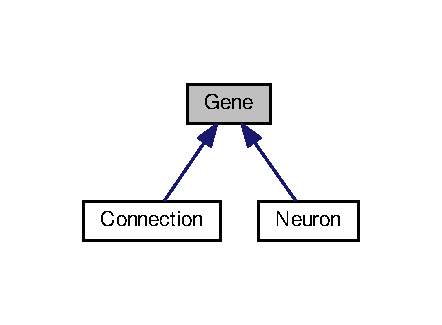
\includegraphics[width=212pt]{classGene__inherit__graph}
\end{center}
\end{figure}


\subsection{Detailed Description}
Class representing gene. 

It stores unique id, allows to clone, and mutate. Provides methods accessible by \hyperlink{classGenotype}{Genotype}. \begin{DoxyAuthor}{Author}
Jakub Fajkowski 
\end{DoxyAuthor}


The documentation for this class was generated from the following files\+:\begin{DoxyCompactItemize}
\item 
src/\+A\+I/Gene.\+h\item 
src/\+A\+I/Gene.\+cc\end{DoxyCompactItemize}

\hypertarget{classGenome}{}\section{Genome Class Reference}
\label{classGenome}\index{Genome@{Genome}}


Represents genome.  




{\ttfamily \#include $<$Genome.\+h$>$}



\subsection{Detailed Description}
Represents genome. 

It consists of two genotypes -\/ one representing Neurons and other representing Connections. It applies specified mutation types (like adding, deleting or modyfing Neuron/\+Connection) It allows crossing with other genome. \begin{DoxyAuthor}{Author}
Jakub Fajkowski 
\end{DoxyAuthor}


The documentation for this class was generated from the following files\+:\begin{DoxyCompactItemize}
\item 
src/\+A\+I/Genome.\+h\item 
src/\+A\+I/Genome.\+cc\end{DoxyCompactItemize}

\hypertarget{classGenotype}{}\section{Genotype$<$ T $>$ Class Template Reference}
\label{classGenotype}\index{Genotype$<$ T $>$@{Genotype$<$ T $>$}}


Represents genotype.  




{\ttfamily \#include $<$Genotype.\+hpp$>$}

\subsection*{Public Member Functions}
\begin{DoxyCompactItemize}
\item 
{\bfseries Genotype} (const \hyperlink{classGenotype}{Genotype} \&genotype)\hypertarget{classGenotype_ae29841aca68c4e2f7ab34f5287aab699}{}\label{classGenotype_ae29841aca68c4e2f7ab34f5287aab699}

\item 
P\+Genotype$<$ T $>$ {\bfseries clone} () const \hypertarget{classGenotype_ae530c5a1420c152ea8c944aec6637ae0}{}\label{classGenotype_ae530c5a1420c152ea8c944aec6637ae0}

\item 
void {\bfseries insert} (const std\+::shared\+\_\+ptr$<$ T $>$ \&gene)\hypertarget{classGenotype_aa49caf873e5c01f7b0c36c0905f83902}{}\label{classGenotype_aa49caf873e5c01f7b0c36c0905f83902}

\item 
bool {\bfseries contains} (const std\+::shared\+\_\+ptr$<$ T $>$ \&gene)\hypertarget{classGenotype_aedc67c3bcfc023c2c3d39bfbe6ac4a97}{}\label{classGenotype_aedc67c3bcfc023c2c3d39bfbe6ac4a97}

\item 
void {\bfseries erase} (const std\+::shared\+\_\+ptr$<$ T $>$ \&gene)\hypertarget{classGenotype_a5970e8399e8d0d725517e23e309a32fb}{}\label{classGenotype_a5970e8399e8d0d725517e23e309a32fb}

\item 
std\+::shared\+\_\+ptr$<$ T $>$ \& {\bfseries operator\mbox{[}$\,$\mbox{]}} (size\+\_\+t index)\hypertarget{classGenotype_a79ab71079ff510e6cf879234d1173882}{}\label{classGenotype_a79ab71079ff510e6cf879234d1173882}

\item 
const std\+::shared\+\_\+ptr$<$ T $>$ \& {\bfseries operator\mbox{[}$\,$\mbox{]}} (size\+\_\+t index) const \hypertarget{classGenotype_aab215e1c057e93b3d986998bdae1f3d9}{}\label{classGenotype_aab215e1c057e93b3d986998bdae1f3d9}

\item 
bool {\bfseries operator==} (const \hyperlink{classGenotype}{Genotype} \&rhs) const \hypertarget{classGenotype_a6b7de41bb91479adc030ee4db3a5aab7}{}\label{classGenotype_a6b7de41bb91479adc030ee4db3a5aab7}

\item 
bool {\bfseries operator!=} (const \hyperlink{classGenotype}{Genotype} \&rhs) const \hypertarget{classGenotype_a9969a19f352b79c2abc10188306071fa}{}\label{classGenotype_a9969a19f352b79c2abc10188306071fa}

\item 
std\+::vector$<$ std\+::shared\+\_\+ptr$<$ T $>$ $>$ {\bfseries get\+Genes} () const \hypertarget{classGenotype_a34bd58f011f915e034ae6b3aea4fd54c}{}\label{classGenotype_a34bd58f011f915e034ae6b3aea4fd54c}

\end{DoxyCompactItemize}
\subsection*{Static Public Member Functions}
\begin{DoxyCompactItemize}
\item 
static P\+Genotype$<$ T $>$ {\bfseries crossover} (\hyperlink{classGenotype}{Genotype} \&parent\+\_\+a, \hyperlink{classGenotype}{Genotype} \&parent\+\_\+b)\hypertarget{classGenotype_a97906c12a2b40c984cb264ee75381f66}{}\label{classGenotype_a97906c12a2b40c984cb264ee75381f66}

\end{DoxyCompactItemize}
\subsection*{Friends}
\begin{DoxyCompactItemize}
\item 
class {\bfseries boost\+::serialization\+::access}\hypertarget{classGenotype_ac98d07dd8f7b70e16ccb9a01abf56b9c}{}\label{classGenotype_ac98d07dd8f7b70e16ccb9a01abf56b9c}

\end{DoxyCompactItemize}


\subsection{Detailed Description}
\subsubsection*{template$<$typename T$>$\\*
class Genotype$<$ T $>$}

Represents genotype. 

It is a collection of unique genes, that are placed by their id. Represents single chain of genes. If there is no gene of specified number it stores nullptr. Provides serialization. \begin{DoxyAuthor}{Author}
Jakub Fajkowski 
\end{DoxyAuthor}


The documentation for this class was generated from the following file\+:\begin{DoxyCompactItemize}
\item 
src/\+A\+I/Genotype.\+hpp\end{DoxyCompactItemize}

\hypertarget{classMachineGamingController_1_1MachineGamingController}{}\section{Machine\+Gaming\+Controller.\+Machine\+Gaming\+Controller Class Reference}
\label{classMachineGamingController_1_1MachineGamingController}\index{Machine\+Gaming\+Controller.\+Machine\+Gaming\+Controller@{Machine\+Gaming\+Controller.\+Machine\+Gaming\+Controller}}
\subsection*{Public Member Functions}
\begin{DoxyCompactItemize}
\item 
def {\bfseries \+\_\+\+\_\+init\+\_\+\+\_\+} (self, stats\+\_\+window)\hypertarget{classMachineGamingController_1_1MachineGamingController_a0552527740e7e5e6a58d2babbe00387a}{}\label{classMachineGamingController_1_1MachineGamingController_a0552527740e7e5e6a58d2babbe00387a}

\item 
def {\bfseries initialize\+\_\+ea} (self, parameters)\hypertarget{classMachineGamingController_1_1MachineGamingController_a7eebd5e59bc078c01bf3057684c54547}{}\label{classMachineGamingController_1_1MachineGamingController_a7eebd5e59bc078c01bf3057684c54547}

\item 
def {\bfseries get\+\_\+current\+\_\+network} (self)\hypertarget{classMachineGamingController_1_1MachineGamingController_aa5f25a8c5bf4cbc0e9dc4f6ad7c1cce5}{}\label{classMachineGamingController_1_1MachineGamingController_aa5f25a8c5bf4cbc0e9dc4f6ad7c1cce5}

\item 
def {\bfseries get\+\_\+current\+\_\+generation} (self)\hypertarget{classMachineGamingController_1_1MachineGamingController_ac90fcf35b4ae810843b5420e1160b0c4}{}\label{classMachineGamingController_1_1MachineGamingController_ac90fcf35b4ae810843b5420e1160b0c4}

\item 
def {\bfseries process} (self)\hypertarget{classMachineGamingController_1_1MachineGamingController_a1bf9bfb9f213daf15538668353af3307}{}\label{classMachineGamingController_1_1MachineGamingController_a1bf9bfb9f213daf15538668353af3307}

\item 
def {\bfseries save} (self, path)\hypertarget{classMachineGamingController_1_1MachineGamingController_a3bfaf926c88d2d4658cac9a31d68cbc5}{}\label{classMachineGamingController_1_1MachineGamingController_a3bfaf926c88d2d4658cac9a31d68cbc5}

\item 
def {\bfseries load} (self, filename)\hypertarget{classMachineGamingController_1_1MachineGamingController_af74b190c4918ace93d1c02d06d95b33c}{}\label{classMachineGamingController_1_1MachineGamingController_af74b190c4918ace93d1c02d06d95b33c}

\item 
def {\bfseries \+\_\+\+\_\+init\+\_\+\+\_\+} (self, stats\+\_\+window)\hypertarget{classMachineGamingController_1_1MachineGamingController_a0552527740e7e5e6a58d2babbe00387a}{}\label{classMachineGamingController_1_1MachineGamingController_a0552527740e7e5e6a58d2babbe00387a}

\item 
def {\bfseries initialize\+\_\+ea} (self, parameters)\hypertarget{classMachineGamingController_1_1MachineGamingController_a7eebd5e59bc078c01bf3057684c54547}{}\label{classMachineGamingController_1_1MachineGamingController_a7eebd5e59bc078c01bf3057684c54547}

\item 
def {\bfseries get\+\_\+current\+\_\+network} (self)\hypertarget{classMachineGamingController_1_1MachineGamingController_aa5f25a8c5bf4cbc0e9dc4f6ad7c1cce5}{}\label{classMachineGamingController_1_1MachineGamingController_aa5f25a8c5bf4cbc0e9dc4f6ad7c1cce5}

\item 
def {\bfseries get\+\_\+current\+\_\+generation} (self)\hypertarget{classMachineGamingController_1_1MachineGamingController_ac90fcf35b4ae810843b5420e1160b0c4}{}\label{classMachineGamingController_1_1MachineGamingController_ac90fcf35b4ae810843b5420e1160b0c4}

\item 
def {\bfseries process} (self)\hypertarget{classMachineGamingController_1_1MachineGamingController_a1bf9bfb9f213daf15538668353af3307}{}\label{classMachineGamingController_1_1MachineGamingController_a1bf9bfb9f213daf15538668353af3307}

\item 
def {\bfseries save} (self, path)\hypertarget{classMachineGamingController_1_1MachineGamingController_a3bfaf926c88d2d4658cac9a31d68cbc5}{}\label{classMachineGamingController_1_1MachineGamingController_a3bfaf926c88d2d4658cac9a31d68cbc5}

\item 
def {\bfseries load} (self, filename)\hypertarget{classMachineGamingController_1_1MachineGamingController_af74b190c4918ace93d1c02d06d95b33c}{}\label{classMachineGamingController_1_1MachineGamingController_af74b190c4918ace93d1c02d06d95b33c}

\end{DoxyCompactItemize}
\subsection*{Public Attributes}
\begin{DoxyCompactItemize}
\item 
{\bfseries stats\+\_\+window}\hypertarget{classMachineGamingController_1_1MachineGamingController_a5c7fa65b5ff61ced3e53b6a75be9b447}{}\label{classMachineGamingController_1_1MachineGamingController_a5c7fa65b5ff61ced3e53b6a75be9b447}

\item 
{\bfseries input\+\_\+size}\hypertarget{classMachineGamingController_1_1MachineGamingController_a5d895aaebf825121920b865c58f1e4a4}{}\label{classMachineGamingController_1_1MachineGamingController_a5d895aaebf825121920b865c58f1e4a4}

\item 
{\bfseries neural\+\_\+network}\hypertarget{classMachineGamingController_1_1MachineGamingController_a3976256fc7d27ebe7d28ec536911d62e}{}\label{classMachineGamingController_1_1MachineGamingController_a3976256fc7d27ebe7d28ec536911d62e}

\item 
{\bfseries ea}\hypertarget{classMachineGamingController_1_1MachineGamingController_afa9b244a5044affb82da318a3334d380}{}\label{classMachineGamingController_1_1MachineGamingController_afa9b244a5044affb82da318a3334d380}

\end{DoxyCompactItemize}


\subsection{Detailed Description}
\begin{DoxyVerb}\end{DoxyVerb}
 

The documentation for this class was generated from the following file\+:\begin{DoxyCompactItemize}
\item 
cmake-\/build-\/debug/src/\+Asteroids/Machine\+Gaming\+Controller.\+py\end{DoxyCompactItemize}

\input{classMachineGamingWindow_1_1MachineGamingWindow}
\hypertarget{classMissile_1_1Missile}{}\section{Missile.\+Missile Class Reference}
\label{classMissile_1_1Missile}\index{Missile.\+Missile@{Missile.\+Missile}}


Inheritance diagram for Missile.\+Missile\+:\nopagebreak
\begin{figure}[H]
\begin{center}
\leavevmode
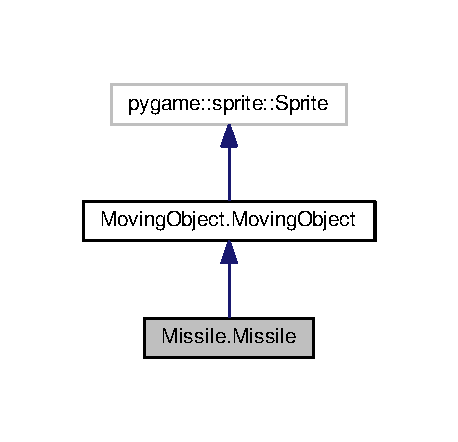
\includegraphics[width=303pt]{classMissile_1_1Missile__inherit__graph}
\end{center}
\end{figure}


Collaboration diagram for Missile.\+Missile\+:\nopagebreak
\begin{figure}[H]
\begin{center}
\leavevmode
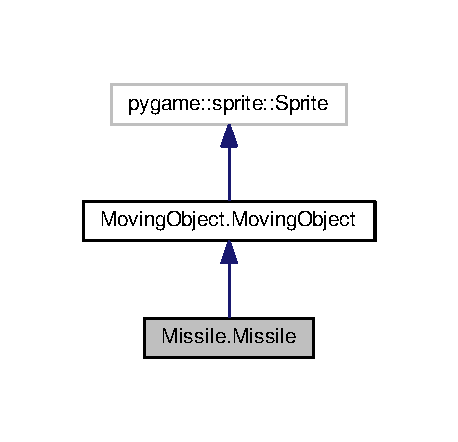
\includegraphics[width=303pt]{classMissile_1_1Missile__coll__graph}
\end{center}
\end{figure}
\subsection*{Public Member Functions}
\begin{DoxyCompactItemize}
\item 
def {\bfseries \+\_\+\+\_\+init\+\_\+\+\_\+} (self, coordinates, velocity=\hyperlink{classVector_1_1Vector}{Vector}(0, 0), direction=0)\hypertarget{classMissile_1_1Missile_acd19b70b0fff20d2d1fb2e18c8455e93}{}\label{classMissile_1_1Missile_acd19b70b0fff20d2d1fb2e18c8455e93}

\item 
def {\bfseries update} (self, surface)\hypertarget{classMissile_1_1Missile_ab1ae0964e6012a269eedb97e906f9d58}{}\label{classMissile_1_1Missile_ab1ae0964e6012a269eedb97e906f9d58}

\item 
def {\bfseries \+\_\+\+\_\+init\+\_\+\+\_\+} (self, coordinates, velocity=\hyperlink{classVector_1_1Vector}{Vector}(0, 0), direction=0)\hypertarget{classMissile_1_1Missile_acd19b70b0fff20d2d1fb2e18c8455e93}{}\label{classMissile_1_1Missile_acd19b70b0fff20d2d1fb2e18c8455e93}

\item 
def {\bfseries update} (self, surface)\hypertarget{classMissile_1_1Missile_ab1ae0964e6012a269eedb97e906f9d58}{}\label{classMissile_1_1Missile_ab1ae0964e6012a269eedb97e906f9d58}

\end{DoxyCompactItemize}
\subsection*{Additional Inherited Members}


The documentation for this class was generated from the following file\+:\begin{DoxyCompactItemize}
\item 
cmake-\/build-\/debug/src/\+Asteroids/Missile.\+py\end{DoxyCompactItemize}

\hypertarget{classMovingObject_1_1MovingObject}{}\section{Moving\+Object.\+Moving\+Object Class Reference}
\label{classMovingObject_1_1MovingObject}\index{Moving\+Object.\+Moving\+Object@{Moving\+Object.\+Moving\+Object}}


Inheritance diagram for Moving\+Object.\+Moving\+Object\+:
\nopagebreak
\begin{figure}[H]
\begin{center}
\leavevmode
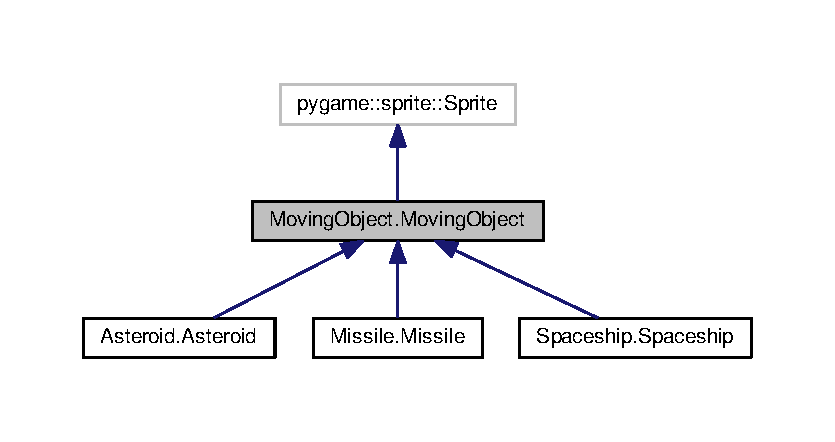
\includegraphics[width=350pt]{classMovingObject_1_1MovingObject__inherit__graph}
\end{center}
\end{figure}


Collaboration diagram for Moving\+Object.\+Moving\+Object\+:
\nopagebreak
\begin{figure}[H]
\begin{center}
\leavevmode
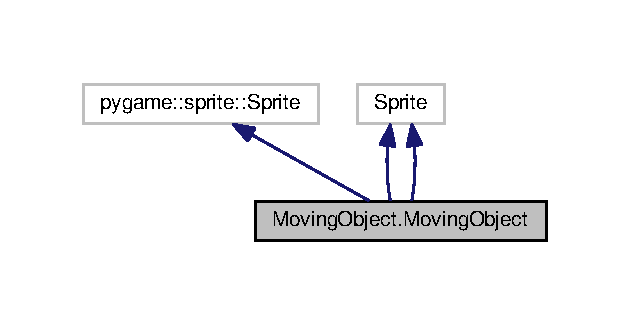
\includegraphics[width=220pt]{classMovingObject_1_1MovingObject__coll__graph}
\end{center}
\end{figure}
\subsection*{Public Member Functions}
\begin{DoxyCompactItemize}
\item 
def {\bfseries \+\_\+\+\_\+init\+\_\+\+\_\+} (self, image, coordinates, does\+\_\+it\+\_\+bounce, velocity=\hyperlink{classVector_1_1Vector}{Vector}(0, 0), direction=0, slows\+\_\+down\+\_\+after\+\_\+bounce=False, image\+\_\+scale=1, listener=None)\hypertarget{classMovingObject_1_1MovingObject_a237013581377a7e5f7163d47254dbce8}{}\label{classMovingObject_1_1MovingObject_a237013581377a7e5f7163d47254dbce8}

\item 
def {\bfseries update} (self, surface)\hypertarget{classMovingObject_1_1MovingObject_ab8d51c9a7e120afad47200b6166d2530}{}\label{classMovingObject_1_1MovingObject_ab8d51c9a7e120afad47200b6166d2530}

\item 
def \hyperlink{classMovingObject_1_1MovingObject_ac2299da57e4ff40983ed385c33ac4c63}{rotate\+\_\+image} (self, angle)
\item 
def {\bfseries move} (self)\hypertarget{classMovingObject_1_1MovingObject_a6060cd55441bc6f9473c4ad5520adc8c}{}\label{classMovingObject_1_1MovingObject_a6060cd55441bc6f9473c4ad5520adc8c}

\item 
def {\bfseries is\+\_\+on\+\_\+screen} (self)\hypertarget{classMovingObject_1_1MovingObject_a3c44ea1a39ee9bd15bb16295a7f6bf75}{}\label{classMovingObject_1_1MovingObject_a3c44ea1a39ee9bd15bb16295a7f6bf75}

\item 
def {\bfseries destroy} (self)\hypertarget{classMovingObject_1_1MovingObject_a7deae65ed90400dab791e8611e86c833}{}\label{classMovingObject_1_1MovingObject_a7deae65ed90400dab791e8611e86c833}

\end{DoxyCompactItemize}
\subsection*{Public Attributes}
\begin{DoxyCompactItemize}
\item 
{\bfseries rect}\hypertarget{classMovingObject_1_1MovingObject_a6e9925838ed3028698c1164d2d763245}{}\label{classMovingObject_1_1MovingObject_a6e9925838ed3028698c1164d2d763245}

\item 
{\bfseries coordinates}\hypertarget{classMovingObject_1_1MovingObject_a4d1309f9d6f6ad8ebe03ce5e14325045}{}\label{classMovingObject_1_1MovingObject_a4d1309f9d6f6ad8ebe03ce5e14325045}

\item 
{\bfseries velocity}\hypertarget{classMovingObject_1_1MovingObject_a7a0d3bf890cd7711bcdbaa2d25c4d0f4}{}\label{classMovingObject_1_1MovingObject_a7a0d3bf890cd7711bcdbaa2d25c4d0f4}

\item 
{\bfseries direction}\hypertarget{classMovingObject_1_1MovingObject_a52cda6e4073bf975ac10d85df1abaa91}{}\label{classMovingObject_1_1MovingObject_a52cda6e4073bf975ac10d85df1abaa91}

\end{DoxyCompactItemize}


\subsection{Member Function Documentation}
\index{Moving\+Object\+::\+Moving\+Object@{Moving\+Object\+::\+Moving\+Object}!rotate\+\_\+image@{rotate\+\_\+image}}
\index{rotate\+\_\+image@{rotate\+\_\+image}!Moving\+Object\+::\+Moving\+Object@{Moving\+Object\+::\+Moving\+Object}}
\subsubsection[{\texorpdfstring{rotate\+\_\+image(self, angle)}{rotate_image(self, angle)}}]{\setlength{\rightskip}{0pt plus 5cm}def Moving\+Object.\+Moving\+Object.\+rotate\+\_\+image (
\begin{DoxyParamCaption}
\item[{}]{self, }
\item[{}]{angle}
\end{DoxyParamCaption}
)}\hypertarget{classMovingObject_1_1MovingObject_ac2299da57e4ff40983ed385c33ac4c63}{}\label{classMovingObject_1_1MovingObject_ac2299da57e4ff40983ed385c33ac4c63}
\begin{DoxyVerb}rotate an image while keeping its center and size\end{DoxyVerb}
 

The documentation for this class was generated from the following file\+:\begin{DoxyCompactItemize}
\item 
src/\+Asteroids/Moving\+Object.\+py\end{DoxyCompactItemize}

\hypertarget{classNeuralNetwork}{}\section{Neural\+Network Class Reference}
\label{classNeuralNetwork}\index{Neural\+Network@{Neural\+Network}}


Represents neural network -\/ multilayer perceptron.  




{\ttfamily \#include $<$Neural\+Network.\+h$>$}

\subsection*{Public Member Functions}
\begin{DoxyCompactItemize}
\item 
{\bfseries Neural\+Network} (int input\+\_\+size, int hidden\+\_\+layers, int output\+\_\+size)\hypertarget{classNeuralNetwork_a246f904545417df2801e56277ab8d53f}{}\label{classNeuralNetwork_a246f904545417df2801e56277ab8d53f}

\item 
{\bfseries Neural\+Network} (const \hyperlink{classNeuralNetwork}{Neural\+Network} \&neural\+\_\+network)\hypertarget{classNeuralNetwork_a9b688c5f00977e83fedea7ee021348f1}{}\label{classNeuralNetwork_a9b688c5f00977e83fedea7ee021348f1}

\item 
{\bfseries Neural\+Network} (const \hyperlink{classGenome}{Genome} \&genome)\hypertarget{classNeuralNetwork_a772972afe658adbb165af9e8b384e552}{}\label{classNeuralNetwork_a772972afe658adbb165af9e8b384e552}

\item 
void {\bfseries mutate} (const Mutation\+Type \&mutation\+\_\+type)\hypertarget{classNeuralNetwork_a95ce793f6206c627f4d436be8348eede}{}\label{classNeuralNetwork_a95ce793f6206c627f4d436be8348eede}

\item 
void {\bfseries randomize\+All\+Weights} ()\hypertarget{classNeuralNetwork_a94e3233f8f2f6c2f1e205b67ddca7adf}{}\label{classNeuralNetwork_a94e3233f8f2f6c2f1e205b67ddca7adf}

\item 
void \hyperlink{classNeuralNetwork_a06a48c985365b4f933d0abe8dc894a1c}{feed\+Forward} (const Matrix \&input)
\item 
const Matrix \& \hyperlink{classNeuralNetwork_a151d07a86bcb717704c3ff8a2f6f35ad}{get\+Output} () const 
\item 
double {\bfseries get\+Fitness} () const \hypertarget{classNeuralNetwork_a6a8e4dfa1a2efcb63a576cac81fb9fe4}{}\label{classNeuralNetwork_a6a8e4dfa1a2efcb63a576cac81fb9fe4}

\item 
void {\bfseries set\+Fitness} (double fitness)\hypertarget{classNeuralNetwork_a9be745ebf5c3f469791439aee1835b0a}{}\label{classNeuralNetwork_a9be745ebf5c3f469791439aee1835b0a}

\item 
bool {\bfseries operator==} (const \hyperlink{classNeuralNetwork}{Neural\+Network} \&rhs) const \hypertarget{classNeuralNetwork_a2a3aff2fe2ee178914a3676ad4c88c51}{}\label{classNeuralNetwork_a2a3aff2fe2ee178914a3676ad4c88c51}

\item 
bool {\bfseries operator!=} (const \hyperlink{classNeuralNetwork}{Neural\+Network} \&rhs) const \hypertarget{classNeuralNetwork_ae5ac2160c59e9b38d551bff997e52645}{}\label{classNeuralNetwork_ae5ac2160c59e9b38d551bff997e52645}

\end{DoxyCompactItemize}
\subsection*{Static Public Member Functions}
\begin{DoxyCompactItemize}
\item 
static bool \hyperlink{classNeuralNetwork_ac6e9655da50b97ca94f4e34bf3de3adc}{compare} (const P\+Neural\+Network \&p1, const P\+Neural\+Network \&p2)
\begin{DoxyCompactList}\small\item\em Fitness comparison. \end{DoxyCompactList}\item 
static P\+Neural\+Network {\bfseries crossover} (\hyperlink{classNeuralNetwork}{Neural\+Network} \&parent\+\_\+a, \hyperlink{classNeuralNetwork}{Neural\+Network} \&parent\+\_\+b)\hypertarget{classNeuralNetwork_a1168869bf81b753ae8b20ea518e11593}{}\label{classNeuralNetwork_a1168869bf81b753ae8b20ea518e11593}

\end{DoxyCompactItemize}
\subsection*{Friends}
\begin{DoxyCompactItemize}
\item 
class {\bfseries boost\+::serialization\+::access}\hypertarget{classNeuralNetwork_ac98d07dd8f7b70e16ccb9a01abf56b9c}{}\label{classNeuralNetwork_ac98d07dd8f7b70e16ccb9a01abf56b9c}

\end{DoxyCompactItemize}


\subsection{Detailed Description}
Represents neural network -\/ multilayer perceptron. 

It provides evolutionary algorithm compatible methods and members. Allows to be crossed-\/over or mutated. Used to predict output by input using unknown function. \begin{DoxyAuthor}{Author}
Jakub Fajkowski 
\end{DoxyAuthor}


\subsection{Member Function Documentation}
\index{Neural\+Network@{Neural\+Network}!compare@{compare}}
\index{compare@{compare}!Neural\+Network@{Neural\+Network}}
\subsubsection[{\texorpdfstring{compare(const P\+Neural\+Network \&p1, const P\+Neural\+Network \&p2)}{compare(const PNeuralNetwork &p1, const PNeuralNetwork &p2)}}]{\setlength{\rightskip}{0pt plus 5cm}bool Neural\+Network\+::compare (
\begin{DoxyParamCaption}
\item[{const P\+Neural\+Network \&}]{p1, }
\item[{const P\+Neural\+Network \&}]{p2}
\end{DoxyParamCaption}
)\hspace{0.3cm}{\ttfamily [static]}}\hypertarget{classNeuralNetwork_ac6e9655da50b97ca94f4e34bf3de3adc}{}\label{classNeuralNetwork_ac6e9655da50b97ca94f4e34bf3de3adc}


Fitness comparison. 

Comparator using neural network fitness. 
\begin{DoxyParams}{Parameters}
{\em neural} & network one \\
\hline
{\em neural} & network two \\
\hline
\end{DoxyParams}
\begin{DoxyReturn}{Returns}
True if p1\textquotesingle{}s fitness is greater than p2\textquotesingle{}s fitness. Else false. 
\end{DoxyReturn}
\index{Neural\+Network@{Neural\+Network}!feed\+Forward@{feed\+Forward}}
\index{feed\+Forward@{feed\+Forward}!Neural\+Network@{Neural\+Network}}
\subsubsection[{\texorpdfstring{feed\+Forward(const Matrix \&input)}{feedForward(const Matrix &input)}}]{\setlength{\rightskip}{0pt plus 5cm}void Neural\+Network\+::feed\+Forward (
\begin{DoxyParamCaption}
\item[{const Matrix \&}]{input}
\end{DoxyParamCaption}
)}\hypertarget{classNeuralNetwork_a06a48c985365b4f933d0abe8dc894a1c}{}\label{classNeuralNetwork_a06a48c985365b4f933d0abe8dc894a1c}
Neural network using provided input calculate some output values. 
\begin{DoxyParams}{Parameters}
{\em input} & vector \\
\hline
\end{DoxyParams}
\index{Neural\+Network@{Neural\+Network}!get\+Output@{get\+Output}}
\index{get\+Output@{get\+Output}!Neural\+Network@{Neural\+Network}}
\subsubsection[{\texorpdfstring{get\+Output() const }{getOutput() const }}]{\setlength{\rightskip}{0pt plus 5cm}const Matrix \& Neural\+Network\+::get\+Output (
\begin{DoxyParamCaption}
{}
\end{DoxyParamCaption}
) const}\hypertarget{classNeuralNetwork_a151d07a86bcb717704c3ff8a2f6f35ad}{}\label{classNeuralNetwork_a151d07a86bcb717704c3ff8a2f6f35ad}
Feed forward method should be called before. \begin{DoxyReturn}{Returns}
Calculated output value. 
\end{DoxyReturn}


The documentation for this class was generated from the following files\+:\begin{DoxyCompactItemize}
\item 
src/\+A\+I/Neural\+Network.\+h\item 
src/\+A\+I/Neural\+Network.\+cc\end{DoxyCompactItemize}

\hypertarget{classNeuralNetworkWrapper}{}\section{Neural\+Network\+Wrapper Class Reference}
\label{classNeuralNetworkWrapper}\index{Neural\+Network\+Wrapper@{Neural\+Network\+Wrapper}}


Wrapper for \hyperlink{classNeuralNetwork}{Neural\+Network}.  




{\ttfamily \#include $<$Neural\+Network\+Wrapper.\+h$>$}

\subsection*{Public Member Functions}
\begin{DoxyCompactItemize}
\item 
{\bfseries Neural\+Network\+Wrapper} (int input\+\_\+size, int hidden\+\_\+layers, int output\+\_\+size)\hypertarget{classNeuralNetworkWrapper_a669dc7ff0b6f17d182bbae149f344f51}{}\label{classNeuralNetworkWrapper_a669dc7ff0b6f17d182bbae149f344f51}

\item 
{\bfseries Neural\+Network\+Wrapper} (P\+Neural\+Network p\+Neural\+Network)\hypertarget{classNeuralNetworkWrapper_a012b510ced2c1c39d0d2df160246cb29}{}\label{classNeuralNetworkWrapper_a012b510ced2c1c39d0d2df160246cb29}

\item 
const py\+::list {\bfseries get\+Output} ()\hypertarget{classNeuralNetworkWrapper_ae16c5f85afd47b5b569020f6f92c9720}{}\label{classNeuralNetworkWrapper_ae16c5f85afd47b5b569020f6f92c9720}

\item 
void {\bfseries feed\+Forward} (py\+::list \&input)\hypertarget{classNeuralNetworkWrapper_a22d7e6ff1fad1ca9c1e654d59114510e}{}\label{classNeuralNetworkWrapper_a22d7e6ff1fad1ca9c1e654d59114510e}

\item 
double {\bfseries get\+Fitness} () const \hypertarget{classNeuralNetworkWrapper_adb481c656d747eb2c028f1fb9f7f71f8}{}\label{classNeuralNetworkWrapper_adb481c656d747eb2c028f1fb9f7f71f8}

\item 
void {\bfseries set\+Fitness} (double fitness)\hypertarget{classNeuralNetworkWrapper_ab8417a449fc7d6693e5f186856a6cbb9}{}\label{classNeuralNetworkWrapper_ab8417a449fc7d6693e5f186856a6cbb9}

\end{DoxyCompactItemize}


\subsection{Detailed Description}
Wrapper for \hyperlink{classNeuralNetwork}{Neural\+Network}. 

It makes \hyperlink{classNeuralNetwork}{Neural\+Network} class public methods fully accessible in Python. \begin{DoxyAuthor}{Author}
Piotr Truszczynski 
\end{DoxyAuthor}


The documentation for this class was generated from the following files\+:\begin{DoxyCompactItemize}
\item 
src/\+A\+I/Neural\+Network\+Wrapper.\+h\item 
src/\+A\+I/Neural\+Network\+Wrapper.\+cc\end{DoxyCompactItemize}

\hypertarget{classNeuron}{}\section{Neuron Class Reference}
\label{classNeuron}\index{Neuron@{Neuron}}


Represents network neurons.  




{\ttfamily \#include $<$Neuron.\+h$>$}



Inheritance diagram for Neuron\+:
\nopagebreak
\begin{figure}[H]
\begin{center}
\leavevmode
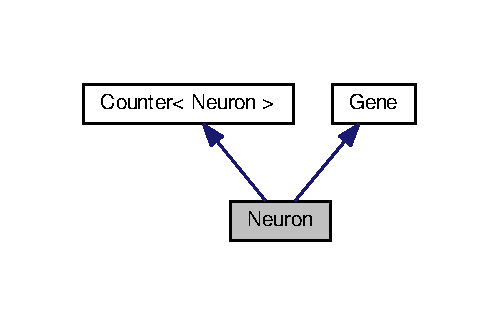
\includegraphics[width=240pt]{classNeuron__inherit__graph}
\end{center}
\end{figure}


Collaboration diagram for Neuron\+:
\nopagebreak
\begin{figure}[H]
\begin{center}
\leavevmode
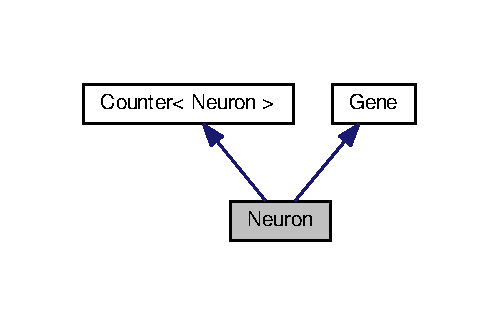
\includegraphics[width=240pt]{classNeuron__coll__graph}
\end{center}
\end{figure}
\subsection*{Public Member Functions}
\begin{DoxyCompactItemize}
\item 
{\bfseries Neuron} (int layer\+\_\+number)\hypertarget{classNeuron_aaaec837656bd4297894e31894976798c}{}\label{classNeuron_aaaec837656bd4297894e31894976798c}

\item 
{\bfseries Neuron} (const \hyperlink{classNeuron}{Neuron} \&neuron)\hypertarget{classNeuron_a03214e3a9896fc827ad081c9ba79da88}{}\label{classNeuron_a03214e3a9896fc827ad081c9ba79da88}

\item 
virtual P\+Gene {\bfseries clone} () const \hypertarget{classNeuron_ad5415199448e7b7c121b6c611251733d}{}\label{classNeuron_ad5415199448e7b7c121b6c611251733d}

\item 
virtual void {\bfseries mutate} (Mutation\+Type mutation\+\_\+type)\hypertarget{classNeuron_a68fd2220abf655ddf5bed07241af2746}{}\label{classNeuron_a68fd2220abf655ddf5bed07241af2746}

\item 
bool {\bfseries operator==} (const \hyperlink{classNeuron}{Neuron} \&rhs) const \hypertarget{classNeuron_a27cbe8fe114357e3b76028b6d6a53ba4}{}\label{classNeuron_a27cbe8fe114357e3b76028b6d6a53ba4}

\item 
bool {\bfseries operator!=} (const \hyperlink{classNeuron}{Neuron} \&rhs) const \hypertarget{classNeuron_a7fa60e1dde3ee05eb8edd238cd718d18}{}\label{classNeuron_a7fa60e1dde3ee05eb8edd238cd718d18}

\item 
int {\bfseries get\+Layer\+Number} () const \hypertarget{classNeuron_a5cd7ad3ac7abda10e8e1c97694139bea}{}\label{classNeuron_a5cd7ad3ac7abda10e8e1c97694139bea}

\end{DoxyCompactItemize}
\subsection*{Friends}
\begin{DoxyCompactItemize}
\item 
class {\bfseries boost\+::serialization\+::access}\hypertarget{classNeuron_ac98d07dd8f7b70e16ccb9a01abf56b9c}{}\label{classNeuron_ac98d07dd8f7b70e16ccb9a01abf56b9c}

\item 
std\+::ostream \& {\bfseries operator$<$$<$} (std\+::ostream \&os, const \hyperlink{classNeuron}{Neuron} \&neuron)\hypertarget{classNeuron_ae5604409859b602533fbbff506a8ccca}{}\label{classNeuron_ae5604409859b602533fbbff506a8ccca}

\end{DoxyCompactItemize}
\subsection*{Additional Inherited Members}


\subsection{Detailed Description}
Represents network neurons. 

It provides \hyperlink{classGene}{Gene} methods. It is stored in \hyperlink{classGenotype}{Genotype} and when needed \hyperlink{classPhenome}{Phenome} connection matrices are built using it. \begin{DoxyAuthor}{Author}
Jakub Fajkowski 
\end{DoxyAuthor}


The documentation for this class was generated from the following files\+:\begin{DoxyCompactItemize}
\item 
src/\+A\+I/Neuron.\+h\item 
src/\+A\+I/Neuron.\+cc\end{DoxyCompactItemize}

\hypertarget{classPhenome}{}\section{Phenome Class Reference}
\label{classPhenome}\index{Phenome@{Phenome}}


Represents phenome.  




{\ttfamily \#include $<$Phenome.\+h$>$}

\subsection*{Public Member Functions}
\begin{DoxyCompactItemize}
\item 
{\bfseries Phenome} (const \hyperlink{classGenome}{Genome} \&genome)\hypertarget{classPhenome_a900e3f448b143b5db3d44d8ff57f07e3}{}\label{classPhenome_a900e3f448b143b5db3d44d8ff57f07e3}

\item 
bool {\bfseries operator==} (const \hyperlink{classPhenome}{Phenome} \&rhs) const \hypertarget{classPhenome_a4aa383a3c22ab02cf4a58d68b83a70b7}{}\label{classPhenome_a4aa383a3c22ab02cf4a58d68b83a70b7}

\item 
bool {\bfseries operator!=} (const \hyperlink{classPhenome}{Phenome} \&rhs) const \hypertarget{classPhenome_a79ecab1c0a34f2f225d367782b72516c}{}\label{classPhenome_a79ecab1c0a34f2f225d367782b72516c}

\item 
std\+::vector$<$ Matrix $>$ \& {\bfseries get\+Neurons} ()\hypertarget{classPhenome_a8188a170ca1f162932a9a90bb8790599}{}\label{classPhenome_a8188a170ca1f162932a9a90bb8790599}

\item 
const std\+::vector$<$ Matrix $>$ \& {\bfseries get\+Weights} () const \hypertarget{classPhenome_af995a7151ac1e461559937889f0c02c9}{}\label{classPhenome_af995a7151ac1e461559937889f0c02c9}

\end{DoxyCompactItemize}
\subsection*{Friends}
\begin{DoxyCompactItemize}
\item 
std\+::ostream \& {\bfseries operator$<$$<$} (std\+::ostream \&os, const \hyperlink{classPhenome}{Phenome} \&phenome)\hypertarget{classPhenome_a34c29d70c5bc8815abcedce0aaf0cfd4}{}\label{classPhenome_a34c29d70c5bc8815abcedce0aaf0cfd4}

\end{DoxyCompactItemize}


\subsection{Detailed Description}
Represents phenome. 

It is simulating the look of individual. In case of neural networks it reads passed genome and using stored information -\/ generates matrices of neurons and connections. \begin{DoxyAuthor}{Author}
Jakub Fajkowski 
\end{DoxyAuthor}


The documentation for this class was generated from the following files\+:\begin{DoxyCompactItemize}
\item 
src/\+A\+I/Phenome.\+h\item 
src/\+A\+I/Phenome.\+cc\end{DoxyCompactItemize}

\hypertarget{classRandom}{}\section{Random Class Reference}
\label{classRandom}\index{Random@{Random}}


Basic random number generator.  




{\ttfamily \#include $<$Random.\+h$>$}



\subsection{Detailed Description}
Basic random number generator. 

It was inspired by C\# like random generator, therefore it is simple and intuitive. \begin{DoxyAuthor}{Author}
Jakub Fajkowski 
\end{DoxyAuthor}


The documentation for this class was generated from the following files\+:\begin{DoxyCompactItemize}
\item 
src/\+A\+I/Random.\+h\item 
src/\+A\+I/Random.\+cc\end{DoxyCompactItemize}

\hypertarget{classSpaceship_1_1Spaceship}{}\section{Spaceship.\+Spaceship Class Reference}
\label{classSpaceship_1_1Spaceship}\index{Spaceship.\+Spaceship@{Spaceship.\+Spaceship}}


Inheritance diagram for Spaceship.\+Spaceship\+:\nopagebreak
\begin{figure}[H]
\begin{center}
\leavevmode
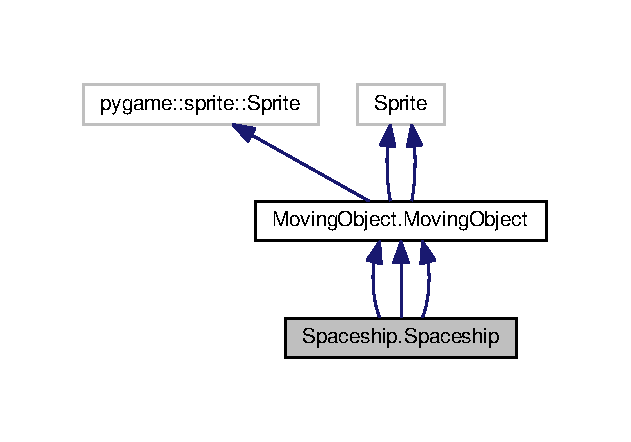
\includegraphics[width=303pt]{classSpaceship_1_1Spaceship__inherit__graph}
\end{center}
\end{figure}


Collaboration diagram for Spaceship.\+Spaceship\+:\nopagebreak
\begin{figure}[H]
\begin{center}
\leavevmode
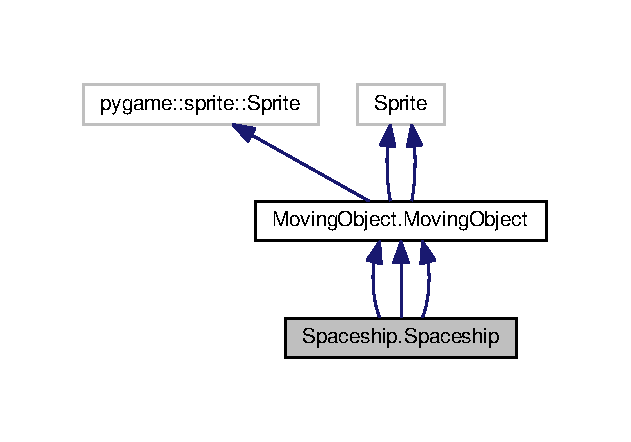
\includegraphics[width=303pt]{classSpaceship_1_1Spaceship__coll__graph}
\end{center}
\end{figure}
\subsection*{Public Member Functions}
\begin{DoxyCompactItemize}
\item 
def {\bfseries \+\_\+\+\_\+init\+\_\+\+\_\+} (self, x, y, listener=None)\hypertarget{classSpaceship_1_1Spaceship_a0ce8d5216e02a15f018cdb852a702a00}{}\label{classSpaceship_1_1Spaceship_a0ce8d5216e02a15f018cdb852a702a00}

\item 
def {\bfseries move} (self)\hypertarget{classSpaceship_1_1Spaceship_a9ed1701b8506b3287a3c0f376965eaa3}{}\label{classSpaceship_1_1Spaceship_a9ed1701b8506b3287a3c0f376965eaa3}

\item 
def {\bfseries steer} (self, key)\hypertarget{classSpaceship_1_1Spaceship_aaad85580a083d4fbb6c839f98224a6c5}{}\label{classSpaceship_1_1Spaceship_aaad85580a083d4fbb6c839f98224a6c5}

\item 
def {\bfseries fire} (self)\hypertarget{classSpaceship_1_1Spaceship_a7cf6faeb7488ab1a77fc5668076c1f35}{}\label{classSpaceship_1_1Spaceship_a7cf6faeb7488ab1a77fc5668076c1f35}

\item 
def {\bfseries \+\_\+\+\_\+init\+\_\+\+\_\+} (self, x, y, listener=None)\hypertarget{classSpaceship_1_1Spaceship_a0ce8d5216e02a15f018cdb852a702a00}{}\label{classSpaceship_1_1Spaceship_a0ce8d5216e02a15f018cdb852a702a00}

\item 
def {\bfseries move} (self)\hypertarget{classSpaceship_1_1Spaceship_a9ed1701b8506b3287a3c0f376965eaa3}{}\label{classSpaceship_1_1Spaceship_a9ed1701b8506b3287a3c0f376965eaa3}

\item 
def {\bfseries steer} (self, key)\hypertarget{classSpaceship_1_1Spaceship_aaad85580a083d4fbb6c839f98224a6c5}{}\label{classSpaceship_1_1Spaceship_aaad85580a083d4fbb6c839f98224a6c5}

\item 
def {\bfseries fire} (self)\hypertarget{classSpaceship_1_1Spaceship_a7cf6faeb7488ab1a77fc5668076c1f35}{}\label{classSpaceship_1_1Spaceship_a7cf6faeb7488ab1a77fc5668076c1f35}

\end{DoxyCompactItemize}
\subsection*{Public Attributes}
\begin{DoxyCompactItemize}
\item 
{\bfseries last\+\_\+shot}\hypertarget{classSpaceship_1_1Spaceship_a56057cc944d63397439253ba0a070fce}{}\label{classSpaceship_1_1Spaceship_a56057cc944d63397439253ba0a070fce}

\item 
{\bfseries direction}\hypertarget{classSpaceship_1_1Spaceship_a8066f1ca4ab44ccd8287634d79607bd6}{}\label{classSpaceship_1_1Spaceship_a8066f1ca4ab44ccd8287634d79607bd6}

\end{DoxyCompactItemize}


The documentation for this class was generated from the following file\+:\begin{DoxyCompactItemize}
\item 
cmake-\/build-\/debug/src/\+Asteroids/Spaceship.\+py\end{DoxyCompactItemize}

\hypertarget{classVector_1_1Vector}{}\section{Vector.\+Vector Class Reference}
\label{classVector_1_1Vector}\index{Vector.\+Vector@{Vector.\+Vector}}
\subsection*{Public Member Functions}
\begin{DoxyCompactItemize}
\item 
def {\bfseries \+\_\+\+\_\+init\+\_\+\+\_\+} (self, x=0, y=0)\hypertarget{classVector_1_1Vector_a53f3e407d6040c60bbb2faa503243218}{}\label{classVector_1_1Vector_a53f3e407d6040c60bbb2faa503243218}

\end{DoxyCompactItemize}
\subsection*{Public Attributes}
\begin{DoxyCompactItemize}
\item 
{\bfseries x}\hypertarget{classVector_1_1Vector_a7f3c3f2b1e0b9e3b97a4f9991a76e0b2}{}\label{classVector_1_1Vector_a7f3c3f2b1e0b9e3b97a4f9991a76e0b2}

\item 
{\bfseries y}\hypertarget{classVector_1_1Vector_a61e9316c753c3d76705841e0d009e4b6}{}\label{classVector_1_1Vector_a61e9316c753c3d76705841e0d009e4b6}

\end{DoxyCompactItemize}


The documentation for this class was generated from the following file\+:\begin{DoxyCompactItemize}
\item 
src/\+Asteroids/Vector.\+py\end{DoxyCompactItemize}

%--- End generated contents ---

% Index
\backmatter
\newpage
\phantomsection
\clearemptydoublepage
\addcontentsline{toc}{chapter}{Index}
\printindex

\end{document}
